\lstdefinestyle{bashstyle}{
    language=bash,
    backgroundcolor = \color{black},
	basicstyle = \color{white}\footnotesize\ttfamily,
	breakatwhitespace=false,         
    breaklines=true,                 
    captionpos=b,                    
    keepspaces=true,                 
    showspaces=false,                
    showstringspaces=false,
    showtabs=false,                  
    tabsize=2,        
    framexleftmargin=6pt,
    framexrightmargin=6pt,
    framextopmargin=6pt,
    framexbottommargin=6pt, 
    frame=tb, 
    framerule=0pt
}
\lstset{style=bashstyle}

\begin{frame}
\section{Tutorial}
\frametitle{Tutorial}
\tableofcontents[currentsection]
\end{frame}

\begin{frame}[fragile]
\subsection{Quickstart}
\frametitle{Quickstart}
\begin{itemize}
\item Download Kafka~\cite{KafkaDownload}
\end{itemize}
\begin{lstlisting}[]
$ tar -xzf kafka_2.11-1.0.0.tgz
$ cd kafka_2.11-1.0.0
\end{lstlisting}

\begin{lstlisting}[]
$ bin/zookeeper-server-start.sh config/zookeeper.properties
$ bin/kafka-server-start.sh config/server.properties
\end{lstlisting}
\end{frame}

\begin{frame}[fragile]
\frametitle{Quickstart}
\begin{lstlisting}[]
$ bin/kafka-topics.sh --create --zookeeper localhost:2181 --replication-factor 1 --partitions 1 --topic test
$ bin/kafka-console-producer.sh --broker-list localhost:9092 --topic test
> This is a message
> This is another message
\end{lstlisting}

\begin{lstlisting}[]
$ bin/kafka-console-consumer.sh --bootstrap-server localhost:9092 --topic test --from-beginning
> This is a message
> This is another message
\end{lstlisting}
\end{frame}

\begin{frame}[fragile]
\subsection{Properties}
\frametitle{Producer Properties}
\begin{table}
{\footnotesize
\begin{tabularx}{\textwidth}{ |X|X|c| } 
\hline 
Name & Beschreibung & Typ \\ \hline \hline
batch-size & Anzahl an Nachrichten die innerhalb eines Batches ins Cluster gepusht werden (asynchrone Kommunikation) & Integer \\ \hline
broker-list/\newline bootstrap.servers & Host- und Portliste zur Verbindung mit dem Cluster & Liste von Strings \\ \hline
message-send-max-retries & Maximale Anzahl an Versuchen das Datum an den Broker zu pushen, bevor der Producer es droped & Integer \\ \hline
topic & Topic unter welches die Daten ins Cluster gepusht werden & String  \\ 
\hline
\end{tabularx}
}
\caption{Beispiele für Producer Properties~\cite{KafkaPropProducer}}
\label{producer_prop}
\end{table}
\begin{center}
\end{center}
\end{frame}

\begin{frame}[fragile]
\frametitle{Consumer Properties}
\begin{table}
{\footnotesize
\begin{tabularx}{\textwidth}{ |X|X|c| } 
\hline 
Name & Beschreibung & Typ \\ \hline \hline
blacklist & Blacklisten von Topics die nicht aboniert werden sollen & Liste von Strings \\ \hline
bootstrap.server/\newline bootstrap.servers & Host und Port zur Verbindung mit dem Cluster & String \\ \hline
from-beginning & Hole die erste Nachricht im Log, sofern der Offset nicht definiert wurde & - \\ \hline
topic & Topic unter welchem die Daten aus dem Cluster geholt werden sollen & String  \\ \hline
whitelist & Whitelisten von Topics die aboniert werden sollen & Liste von Strings \\ 
\hline
\end{tabularx}
}
\caption{Beispiele Consumer Properties~\cite{KafkaPropConsumer}}
\label{consumer_prop}
\end{table}
\begin{center}
\end{center}
\end{frame}

\begin{frame}[fragile]
\frametitle{Weitere Properties}
\begin{itemize}
\item Broker Properties~\cite{KafkaPropBroker}
\item Streams Properties~\cite{KafkaPropStreams}
\item Topic Properties~\cite{KafkaPropTopic}
\item Connect Config Properties~\cite{KafkaPropConnectConfig}
\item AdminClient Properties~\cite{KafkaPropAdminClient}
\end{itemize}
\end{frame}

\begin{frame}[fragile]
\subsection{Kafka Clients}
\frametitle{Kafka Clients}
\begin{itemize}
\item Diverse Clients vorhanden~\cite{KafkaClients}
\begin{itemize}
\item Java, Python, Go, C/C++, .NET, Ruby, ...
\end{itemize}
\item Kafka in Java geschrieben, daher der meiste Support

\end{itemize}
\end{frame}

\begin{frame}[fragile]
\subsection{Twitter App}
\frametitle{Twitter App~\cite{GithubRepo}}
\begin{figure}
\centering
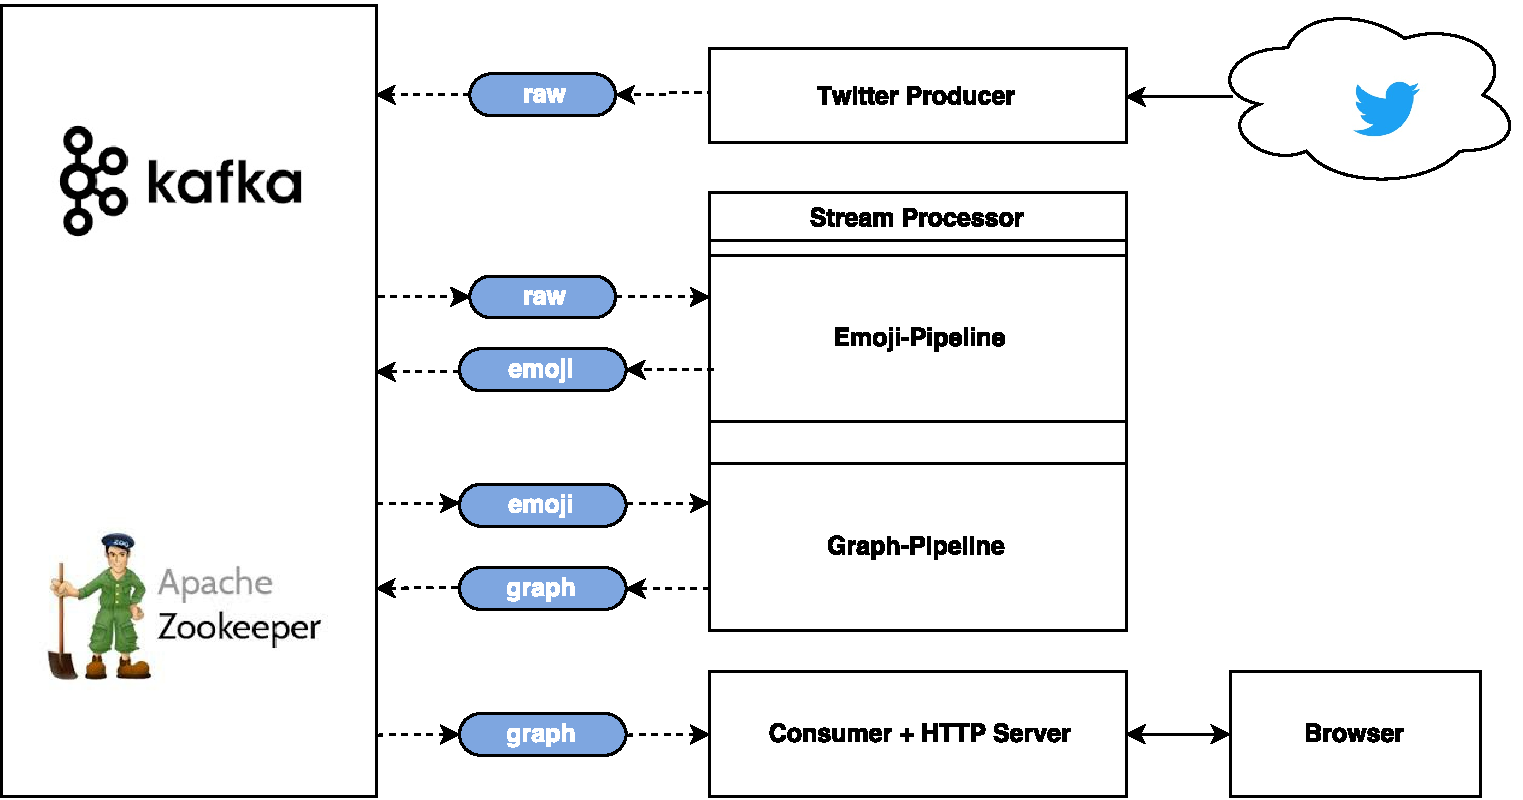
\includegraphics[width=0.95\textwidth]{figure/kafka_tut_diagram.pdf}
\caption{Architektur Twitter App}
\end{figure}
\end{frame}

\definecolor{codegreen}{rgb}{0,0.6,0}
\definecolor{codegray}{rgb}{0.5,0.5,0.5}
\definecolor{codepurple}{rgb}{0.58,0,0.82}
\definecolor{backcolour}{rgb}{0.95,0.95,0.92}
 
\lstdefinestyle{pythonstyle}{
	language=Python,
    basicstyle=\scriptsize\ttfamily,
	backgroundcolor=\color{backcolour},   
    commentstyle=\color{codegreen},
    keywordstyle=\color{magenta},
    numberstyle=\tiny\color{codegray},
    stringstyle=\color{codepurple},
    breakatwhitespace=false,         
    breaklines=true,                 
    captionpos=b,                    
    keepspaces=true,                 
    showspaces=false,                
    showstringspaces=false,
    showtabs=false,                  
    tabsize=2,        
    framexleftmargin=6pt,
    framexrightmargin=6pt,
    framextopmargin=6pt,
    framexbottommargin=6pt, 
    frame=tb, 
    framerule=0pt
}
\lstset{style=pythonstyle}
\begin{frame}[fragile]
\frametitle{Python Producer}
\lstinputlisting[
basicstyle=\scriptsize\ttfamily,
caption=Python Producer]{snippets/snippet-producer.py}
\end{frame}

\begin{frame}[fragile]
\frametitle{Python Processor}
\lstinputlisting[
caption=Python Processor]{snippets/snippet-processor.py}
\end{frame}

\begin{frame}[fragile]
\frametitle{Python Consumer}
\lstinputlisting[
caption=Python Consumer]{snippets/snippet-consumer.py}
\end{frame}

\begin{frame}[fragile]
\frametitle{Screencast}
\begin{center}
\Large{Screencast Demo}
\end{center}
\end{frame}

\begin{frame}
\frametitle{Fragen}
\begin{center}
\Large{Vielen Dank für Eure Aufmerksamkeit!
\\Gibt es Fragen?}
\end{center}
\end{frame}